\documentclass[12pt]{report}

% --- PACKAGES ---
\usepackage[utf8]{inputenc}
\usepackage{times} % Times New Roman
\usepackage[a4paper, margin=1in]{geometry}
\usepackage{setspace}
\usepackage{titlesec}
\usepackage{caption}
\usepackage{enumitem}
\usepackage{graphicx}
\usepackage{indentfirst}
\usepackage{url}     % For URLs in bibliography
\usepackage{textcomp}  % For special symbols
\usepackage[super]{cite}    % For superscript citations
\makeatletter
\renewcommand\@citess[1]{\textsuperscript{[#1]}}
\makeatother

% --- STRICT PLACEMENT & DETAILED BLOCK DIAGRAMS ---
\usepackage{float}
\usepackage{tikz}
\usetikzlibrary{shapes.geometric, arrows.meta, positioning, calc}

% --- DOUBLE SPACING & JUSTIFICATION ---
\doublespacing
\sloppy
\setlength{\parskip}{12pt}
\setlength{\parindent}{0pt}

% --- CHAPTER TITLE FORMAT (16pt, BOLD, CAPS, CENTER) ---
\titleformat{\chapter}[display]
 {\setlength{\parskip}{0pt}\singlespacing\bfseries\fontsize{16}{19}\selectfont\centering}
 {\MakeUppercase{\chaptertitlename\ \thechapter}}
 {19pt}
 {\MakeUppercase}
\titlespacing*{\chapter}{0pt}{-20pt}{12pt}

% --- SECTION FORMAT (14pt, BOLD, CAPS) ---
\titleformat{\section}
 {\bfseries\fontsize{14}{17}\selectfont}
 {\thesection}
 {1em}
 {\MakeUppercase}
\titlespacing*{\section}{0pt}{12pt}{0pt}

% --- SUBSECTION FORMAT (12pt, BOLD) ---
\titleformat{\subsection}
 {\bfseries\fontsize{12}{14}\selectfont}
 {\thesubsection}
 {1em}
 {}
\titlespacing*{\subsection}{0pt}{12pt}{0pt}

% --- SUBSUBSECTION FORMAT (12pt, BOLD) ---
\setcounter{secnumdepth}{3}
\setcounter{tocdepth}{3}
\titleformat{\subsubsection}
 {\bfseries\fontsize{12}{14}\selectfont}
 {\thesubsubsection}
 {1em}
 {}
\titlespacing*{\subsubsection}{0pt}{12pt}{0pt}

% --- CAPTION SETTINGS ---
\captionsetup[table]{position=above, labelfont={normalfont,normalsize}, textfont={normalfont,normalsize}, justification=centering}
\captionsetup[figure]{position=below, labelfont={normalfont,normalsize}, textfont={normalfont,normalsize}, justification=centering}

% --- DOCUMENT START ---
\begin{document}



% ================= TITLE PAGE =================
\thispagestyle{empty}
\begin{center}

\textbf{\Large RAJIV GANDHI INSTITUTE OF TECHNOLOGY}\\[1em]
\textbf{\Large GOVERNMENT ENGINEERING COLLEGE}\\[1em]
\textbf{\large KOTTAYAM - 686 501}\\[1em]

\includegraphics[width=2 cm]{collegelogo.jpg}\\[2em] % Replace with actual logo file

\textbf{\large DEPARTMENT OF COMPUTER APPLICATIONS}\\[1em]
\text{20MCA246 - MAIN PROJECT REPORT}\\[2em]

\textbf{\large AI ENABLED HOME PLANNING \& 3D VISUALISATION\\ WEB APPLICATION}
\\[2em]

Submitted By\\[0.5em]
\textbf{LEKSHMI R RAJAN}\\[0.5em]
\textbf{KTE24MCA-2035}\\[2em]
Under the Guidance of\\[0.5em]
\textbf{Prof. SHILPA M THOMAS}\\[1em]

\includegraphics[width=2 cm]{ktu.jpg}\\[2em] % Replace with actual KTU logo file
\text{APJ ABDUL KALAM TECHNOLOGICAL UNIVERSITY}\\[0.5em]
\text{THIRUVANANTHAPURAM}\\[0.5em]
\text{March 2026}

\end{center}

\newpage
\thispagestyle{empty}
\baselineskip=22.5pt plus .5pt minus .2 pt
\begin{center}
   
    \large{\textbf{DEPARTMENT OF COMPUTER APPLICATIONS}} \\ \vspace{0.9cm}
    \Large{\textbf{RAJIV GANDHI INSTITUTE OF TECHNOLOGY}}\\
    \Large\textbf{KOTTAYAM} \vspace{0.8cm}
    \hspace{2pt}
    
    
    \includegraphics[height=40mm]{collegelogo.jpg}\\
   \vspace{1.5cm}

   \large{\textbf{CERTIFICATE}}
\end{center}
  This is to certify that the project entitled \textbf{ `` AI-ENABLED HOME PLANNING \& 3D VISUALIZATION WEB APPLICATION '' } is a bonafide work carried out by \textbf{Lekshmi R Rajan} (Register No: \textbf{KTE24MCA-2035}) during the academic year \textbf{2025 - 2026} in partial fulfillment of the requirements for the award of the degree of \textbf{Master of Computer Applications} of \textbf{APJ Abdul Kalam Technological University, Thiruvananthapuram, Kerala.}
  
\vspace{3cm}
\hspace{-1.3em}\textbf{Guide}   \hfill \textbf{Head of Department}

\vspace{2cm}

\clearpage
\pagestyle{plain}
\pagenumbering{roman}
% --------------- Declaration page -----------------------%
\addcontentsline{toc}{chapter}{DECLARATION}
\pagenumbering{roman} \setcounter{page}{1}
\begin{center}
{\Large{\bf{DECLARATION}}}
\end{center}

\noindent
 \hspace{.5cm}I, undersigned hereby declare that the project report entitled \textbf {`` AI-ENABLED HOME PLANNING \& 3D VISUALIZATION WEB APPLICATION ''}, submitted for partial fulfillment of the requirements for the award of the degree of Master of Computer Applications of the APJ Abdul Kalam Technological University, Kerala is a bonafide work done by me under the supervision of my guide,  
 \textbf {Prof. SHILPA M THOMAS } . This submission represents my ideas in my own words and where ideas or words of others have been included, I have adequately and accurately cited and referenced the original sources. I also declare that I have adhered to the ethics of academic honesty and integrity and have not misrepresented or fabricated any data or idea or fact or source in my submission. I understand that any violation of the above will be a cause for disciplinary action by the institute and / or the University and can also evoke penal action from the sources which have thus not been properly cited or from whom proper permission has not been obtained. This report has not been previously formed as the basis for the award of any degree, diploma, or similar title of any other University.
\vspace{4cm}

\noindent Place: Kottayam 

\noindent Date: 31/03/2026 \hfill \textbf{LEKSHMI R RAJAN}

\clearpage

\chapter*{ACKNOWLEDGEMENT}
\addcontentsline{toc}{chapter}{ACKNOWLEDGEMENT}

\par I would like to express my sincere gratitude to everyone who has supported me throughout this endeavour. First and foremost, I thank God Almighty for His mercy and blessings; without His guidance, this work would have remained only a dream.

\par I sincerely thank \textbf{Dr. Prince A}, Principal, Rajiv Gandhi Institute of Technology, Kottayam, for providing a conducive environment for the successful completion of this project.

\par I express my deep sense of gratitude to \textbf{Dr. Vineetha S}, Head of the Department of Computer Applications, for granting permission and providing all the necessary facilities to complete this project.

\par I would like to extend my heartfelt thanks to my project guide, \textbf{Prof. Shilpa M Thomas}, for her invaluable guidance, constant support, and encouragement throughout the course of this work. Her constructive suggestions and insightful feedback greatly improved the quality of this project.

\par I also sincerely thank the coordinators, \textbf{Dr. Sangeetha Jose} and \textbf{Dr. Vineetha S}, for their support, guidance, and coordination during the project period.

\par Finally, I would like to express my gratitude to all the faculty members and technical staff of the Department of Computer Applications for their support and assistance.



\vspace{.8in}
\hspace{3.8in}
\noindent \textbf{LEKSHMI R RAJAN}


\chapter*{ABSTRACT}
\addcontentsline{toc}{chapter}{ABSTRACT}
\onehalfspacing
\setlength{\parskip}{1em}
\setlength{\parindent}{0pt}

\textbf{AI-Enabled Home Planning and 3D Visualization Web Application} is an innovative, fully integrated architectural prototyping system designed to revolutionize the early-stage residential design process by addressing the inefficiencies, ambiguities, and manual complexities that plague traditional floor planning workflows. In many architectural scenarios, manual sketching, slow CAD re-tracing, and fragmented cost estimation lead to significant delays, data silos, and spatial misunderstandings, ultimately frustrating both clients and professionals. AI Home Planner eliminates these challenges by offering a unified, multimodal digital solution that seamlessly connects all design phases\-sketch interpretation, semantic segmentation, 3D visualization, and financial forecasting\-within a single, secure, and user-friendly platform. Developed using React.js for a dynamic, responsive, and glassmorphic frontend, FastAPI for a high-concurrency and secure backend framework, and SQLite for reliable and scalable database management, the system ensures data integrity, performance, and smooth interoperability across modules. One of the standout features of the platform is its hybrid AI vision pipeline, which utilizes OpenCV preprocessing to stabilize noisy sketches and a PyTorch-implemented U-Net for precise pixel-level structural wall extraction, allowing users to move effortlessly from paper drawings to interactive WebGL-based 3D environments without the need for manual digitization. The integration of a Scikit-Learn Random Forest regression engine provides real-time predictive construction cost modeling based on extracted spatial dimensions and localized material datasets, simplifying the budgeting process for developers and homeowners alike. Furthermore, the platform incorporates a Groq-powered conversational AI assistant that leverages the extracted geometric JSON to provide contextually aware architectural advice and design optimizations. To maintain security and project privacy, the system employs OAuth2/JWT-based role-based access control (RBAC), ensuring that users and administrators have permissioned access aligned with their needs, thereby protecting sensitive project metadata in compliance with design standards. Overall, the AI Home Planner redefines conceptual residential planning by combining innovation, automation, and deep learning to deliver a comprehensive, scalable, and intelligent architectural ecosystem that enhances user satisfaction, improves design quality, optimizes financial planning, and paves the way toward a future-ready, digital-first smart construction landscape that meets the evolving demands of today’s technology-driven world.

\textbf{Keywords:} AI-Enabled Home Planning, U-Net Segmentation, Computer Vision, 3D Visualization, WebGL, Cost Prediction, Multimodal AI, Architectural Prototyping.



% ================= TOC =================
\tableofcontents
\newpage
\listoffigures
\newpage
\listoftables

% ================= ABBREVIATIONS =================
\begin{center}
\chapter*{LIST OF ABBREVIATIONS}
\addcontentsline{toc}{chapter}{List of Abbreviations}

\begin{spacing}{1.5}                        % Double spacing
\begin{tabular}{p{4cm} p{10cm}} 
\textbf{Abbreviation} & \textbf{Definition} \\
\textbf{AI} & Artificial Intelligence \\
\textbf{ML} & Machine Learning \\
\textbf{DL} & Deep Learning \\
\textbf{CV} & Computer Vision \\
\textbf{API} & Application Programming Interface \\
\textbf{JSON} & JavaScript Object Notation \\
\textbf{BIM} & Building Information Modeling \\
\textbf{WebGL} & Web Graphics Library \\
\textbf{mIoU} & Mean Intersection over Union \\
\textbf{MAE} & Mean Absolute Error \\
\textbf{LLM} & Large Language Model \\
\textbf{CAD} & Computer-Aided Design \\
\textbf{AR} & Augmented Reality \\
\textbf{SRS} & Software Requirements Specification \\
\textbf{JWT} & JSON Web Token \\
\textbf{REST} & Representational State Transfer \\
\textbf{ASGI} & Asynchronous Server Gateway Interface \\
\end{tabular}
\end{spacing}
\end{center}

\newpage
\newcounter{savepage}
\setcounter{savepage}{\value{page}}

% ================= CHAPTER 1 =================
\clearpage
\pagenumbering{arabic}
\chapter{INTRODUCTION}

The project titled AI-Enabled Home Planning and 3D Visualization Web Application focuses on providing an interactive, intelligent, and user-friendly solution for early-stage residential home planning. The system aims to bridge the gap between conceptual house layouts and realistic visualization by using a multimodal artificial intelligence framework to convert 2D hand-drawn sketches into structured three-dimensional (3D) representations\cite{liu2017, chen2019}. By leveraging modern web technologies alongside advanced deep learning models including an OpenCV preprocessing pipeline\cite{opencv2024}, a PyTorch-implemented U-Net for semantic segmentation\cite{ronneberger2015}, and Scikit-Learn for real-time cost estimation\cite{sklearn2024} the project enables users to better understand spatial arrangements, room layouts, and the financial implications of their designs\cite{wang2020}. Furthermore, the integration of a Groq-powered conversational AI chatbot\cite{groq2024} improves clarity, supports informed decision-making, and drastically reduces the dependency on professional architectural tools during the initial planning phase\cite{brown2020}. Additionally, the platform facilitates dynamic spatial optimization and real-time material selection, allowing users to iterate on their architectural concepts with data-driven precision. Such an integrated approach ensures that the transition from a creative sketch to a technically feasible 3D model is both seamless and intuitive, bridging the gap between artistic ideation and professional engineering standards.


\section{Need for Project}

Home planning is a crucial phase in residential construction, where a clear understanding of space utilization, room arrangement, and functionality is essential\cite{eastman2018}. In most cases, early-stage house designs begin with hand-sketched plans, which are inherently ambiguous and difficult for both traditional algorithms and non-technical users to visualize accurately\cite{ahmed2018}. Translating these irregular sketches into realistic, interactive 3D spaces traditionally requires manual re-drawing within complex and fragmented software suites\cite{eastman2018}.

Existing architectural design tools, such as professional CAD software, although powerful, are complex, expensive, and demand specialized training\cite{eastman2018}. Furthermore, existing pipelines separate the sketching phase from visual rendering and financial budgeting\cite{wang2020}. With the advancements in Computer Vision, Deep Learning, and Large Language Models\cite{ronneberger2015, liu2017, vaswani2017}, there is a growing need for an integrated platform that automates this workflow. The proposed project addresses this need by providing an accessible, multi-stage web application that unifies sketch interpretation, 3D visualization, automated cost forecasting, and intelligent conversational assistance in a single ecosystem\cite{brown2020, fastapi2024}.

\section{Objective}

The primary objective of this project is to design, develop, and deliver a fully functional, AI-enabled web application that assists users in estimating costs and visualizing residential house layouts in three dimensions. The specific objectives are:

\subsection{Specific Objectives}

\begin{itemize}
  \item To provide a simple web interface for uploading conceptual hand-drawn floor plans.
  \item To automate the extraction and vectorization of structural walls from sketches using OpenCV and PyTorch U-Net semantic segmentation\cite{opencv2024, ronneberger2015}.
  \item To generate an interactive WebGL-based 3D visualization of the house layout, allowing user interaction through rotation, zoom, and panning\cite{threejs2024}.
  \item To represent functional areas exactly (such as living room, bedroom, kitchen, bathroom, work area, and car porch) via an intermediate geometric JSON mapping\cite{liu2017}.
  \item To execute real-time construction cost estimation using a Scikit-Learn regression model analyzing extracted spatial dimensions\cite{sklearn2024, wang2020}.
  \item To empower users with an integrated conversational AI assistant (Groq LLM) for grounded, context-aware design advice\cite{groq2024, brown2020}.
\end{itemize}

\section{Scope of the Project}

The scope of the project focuses on conceptual residential home planning through a unified, full-stack digital pipeline encompassing layout extraction, visualization, and economic forecasting\cite{eastman2018}.

\subsection{Project Scope}

\begin{itemize}
  \item Development of a high-performance web-based application utilizing FastAPI for coordinating concurrent AI inference processes\cite{fastapi2024}.
  \item Implementation of a hybrid vision pipeline utilizing OpenCV for image noise reduction\cite{opencv2024} and deep learning for robust structural feature extraction\cite{ronneberger2015}.
  \item Generation of interactive 3D visualizations inside the browser from 2D coordinates\cite{threejs2024}, distinguishing rooms with distinct identifiers to improve spatial layout understanding.
  \item Integration of predictive financial analytics, computing materials and labor costs automatically without manual area inputs via Scikit-Learn algorithms\cite{sklearn2024, wang2020}.
  \item Delivery of multimodal conversational interactions, allowing an integrated Chatbot to leverage the geometric JSON data to offer personalized architectural suggestions\cite{groq2024, vaswani2017}.
\end{itemize}

The scope of this project is limited to conceptual home planning and visualization for academic and early-stage design purposes. While providing robust structural recognition, it does not aim to replace professional architectural certification software\cite{eastman2018}. Strict structural load analysis, legal compliance checking, and construction-grade BIM (Building Information Modeling) exports remain out of scope for the current system.

\section{Organization of Thesis}

This report is organized as follows:

\begin{itemize}
  \item \textbf{Chapter 1 -- Introduction:} Presents the background, need, objectives, scope, and organizational structure of the report.
  \item \textbf{Chapter 2 -- Literature Review:} Discusses existing CAD systems, research into computer vision architectures, and gaps within modern architectural software that necessitate this framework.
  \item \textbf{Chapter 3 -- Proposed Methodology:} Details the tools, system architecture design, and step-by-step implementation including OpenCV, PyTorch U-Net, Scikit-Learn, and Groq LLM integration.
  \item \textbf{Chapter 4 -- Results and Analysis:} Presents qualitative segmentation outcomes, comparative cost model benchmarks, and end-to-end processing latency results.
  \item \textbf{Chapter 5 -- Conclusion:} Summarizes the project achievements and validates the fulfillment of all defined objectives.
  \item \textbf{Chapter 6 -- Future Scope:} Suggests extensions such as AR visualization, YOLO-based object detection, BIM export, and real-time collaborative design.
\end{itemize}

% ================= CHAPTER 2 =================
\chapter{LITERATURE REVIEW}

This chapter presents a review of existing systems, tools, and research studies related to residential home planning, computational architecture, and multi-disciplinary AI technologies. It examines traditional professional methodologies, early visual-processing frameworks, and integrated conversational models. The purpose of this review is to understand current capabilities, pinpoint critical functional limitations, and demonstrate how our integrated AI-enabled framework resolves these contemporary industry bottlenecks. 

Historically, the transition from manual drafting to Computer-Aided Design (CAD) revolutionized architectural precision but maintained a high technical barrier for non-professional users. While contemporary BIM (Building Information Modeling) tools offer unparalleled detail, they often lack the intuitive interface required for early-stage conceptual ideation\cite{opencv2024, canny1986}. Recent developments in the AEC (Architecture, Engineering, and Construction) industry have begun to explore deep learning for automated floor plan generation, yet a significant gap remains in translating unstructured human input\—such as hand-drawn sketches\—into precise, actionable geometric data. 

Furthermore, while Large Language Models (LLMs) have transformed natural language interaction, their application in spatial reasoning and structural constraints is still an emerging frontier. By synthesizing these disparate fields, this review establishes a theoretical groundwork for a hybrid system that treats architectural design as a collaborative, multimodal dialogue. The following sections categorize the state-of-the-art into three primary domains: conventional architectural software, computer-vision-based floor plan analysis, and the burgeoning field of generative architectural agents.

\section{Existing System}

Existing home planning systems predominantly rely on traditional approaches or high-end Computer-Aided Design (CAD) tools such as AutoCAD, Revit, and SketchUp. These tools remain the standard for producing accurate, compliance-ready architectural drafting. However, they lack semantic visual intelligence; they require exact manual inputs and cannot interpret the stochastic, noisy lines characteristic of early conceptual hand-sketches. Consequently, architects and clients cannot fluidly transform casual sketches into functional digital equivalents without laborious re-tracing\cite{wang2020} .
Moreover, the existing ecosystem is heavily fragmented. Separate systems manage differing stages of the prototyping loop: one for visualization, another separate spreadsheet framework for cost projection, and third-party personnel to advise on design rules. Web platforms demonstrating basic 3D rendering typically depend heavily on drag-and-drop templates rather than machine reading capabilities, keeping users dependent on multiple disjointed systems.This mechanical rigidity creates a profound "semantic gap" where the software understands the geometry\—vectors, vertices, and layers\—but remains oblivious to the architectural intent. Within traditional CAD environments, a line represents a mathematical distance rather than a structural element with inherent properties like thermal resistance, load-bearing capacity, or cost-per-square-meter. Consequently, any intelligence regarding the "meaning" of the space must be manually injected by a human expert, rendering the software a passive drafting table rather than an active design partner.
Furthermore, the lack of a unified data backbone results in persistent "information silos." When a design modification is made in a visualization tool, the corresponding impact on material procurement, structural integrity, and local building code compliance must be recalculated across disconnected spreadsheets or secondary software modules. This manual synthesis of data across disparate platforms introduces significant latency in the design-to-validation cycle, often leading to costly errors and misaligned expectations between the client and the architect.
The barrier to entry also remains prohibitively high; the steep learning curve associated with parametric modeling often forces users into a "template-driven" workflow. In these scenarios, creative freedom is sacrificed for software convenience, as users are restricted to pre-defined libraries of objects that may not align with their unique spatial visions. There is a clear and urgent need for a "design-first" interface\—one that can perceive the raw intuition of a hand-drawn stroke and autonomously bridge the gap between a conceptual sketch and a multifaceted, data-rich architectural model.

\section{Study on Existing System}

Several research studies have attempted to computationally bridge the gap between 2D layouts and digital formats. Early studies favored algorithms like the Hough Transform\cite{ahmed2018} for extracting structural lines from floor plans. However, these classical vision methods struggled with the irregularities in hand-drawn imagery.
A major breakthrough in addressing these inconsistencies arrived with deep learningspecifically the U-Net architecture\cite{ronneberger2015}, which established a robust approach for exact pixel-level segmentation. Furthermore, frameworks such as FloorNet\cite{liu2017} applied multi-branch CNNs directly towards 3D transformation. Despite their impressive accuracy, these solutions are often computationally dense, lack an interactive user-facing web tool, and do not interpret spatial logic toward external practicalities like financial forecasting.

Separately, studies optimizing construction estimates via machine learning\cite{wang2020} demonstrated that regression algorithms can tightly predict building costs based on geographical dimensions. Yet, these models have remained standalone, continuing to demand that users quantify and input project areas manually.This lack of connectivity between visual perception and economic modeling represents a significant "knowledge gap" in current architectural AI research. While a U-Net may successfully identify a wall boundary, it rarely understands the financial or structural implications of that wall's material composition or its impact on the total project budget. Furthermore, existing end-to-end systems often neglect the "Human-in-the-Loop" aspect, failing to provide an intuitive interface where a non-expert can interactively refine AI-generated outputs.
Most research-grade models also require high-performance localized computing environments, making them inaccessible for real-time deployment on lightweight web-based platforms used by the general public. Consequently, there is a clear demand for a hybrid architecture that not only automates spatial vectorization but also bridges the semantic divide between raw geometry and actionable business intelligencecite{opencv2024}. By synthesizing deep learning, topological simplification, and real-time regression analysis, the need for a unified environment becomes evident\—one where a single sketch can trigger a chain of multi-disciplinary inferences. Our proposed framework addresses these deficiencies by consolidating these fragmented breakthroughs into a singular, browser-accessible architectural agent.

\section{Recent Advancements in Deep Learning for Architectural Analysis}

The field of automatic floor plan analysis has undergone explosive growth due to advancements in machine learning\cite{threejs2024}. Modern architectures like DeepFloorPlan\cite{liu2017} leverage geometry-aware convolutional neural networks to perform real-time recognition of room boundaries and structural elements with high precision. Recent studies have also explored identifying connection points, such as wall corners and door endpoints, using CNNs to establish robust topological links\cite{liu2017}. These data-driven approaches significantly outperform traditional heuristic methods by adapting to varied drawing styles and noise levels.

\section{Machine Learning for Construction Economics}

Accurate cost estimation is critical to the feasibility of any construction project. Traditional estimation methods often struggle with the nonlinear relationships within construction data, leading to frequent cost overruns\cite{liu2017, threejs2024}.. Recent research highlights the effectiveness of ensemble learning techniques, such as Random Forest and XGBoost, in providing more reliable cost predictions during the early design phases. These models enable the processing of large datasets of historical construction costs against extracted spatial metrics, yielding predictive accuracies exceeding 90\% in controlled benchmarks.

\section{Multimodal AI and Conversational Interfaces in Design}

The integration of Large Language Models (LLMs) and multimodal AI has introduced a new paradigm of interactive architectural assistance. By utilizing Transformer-based architectures, systems can now interpret complex design instructions and provide contextually grounded suggestions. Multimodal models, such as CLIP, further enable the alignment of visual geometry with natural language, allowing for seamless communication between users and digital design environments.cite{opencv2024} This shift towards ``Explanatory AI'' ensures that architectural tools are not only generative but also collaborative and informative.

\section{Gap Identification}

Based on the detailed study of existing tools and modern computational architectures, the following gaps have been identified:

\begin{itemize}
  \item \textbf{Lack of Integrated Multimodal Systems:} Separation of visualization systems from construction cost estimation and structural recognition forces users to transition between independently operated tools.
  \item \textbf{Inadequate Tolerance for Abstract Inputs:} Current consumer modeling tools demand explicit layout declarations and fail to interpret the natural variance present in hand-sketched home plans.
  \item \textbf{Absence of Real-Time Predictive Costing within Renderers:} Users currently cannot draw an internal wall manually and subsequently receive automated real-time updates regarding architectural expenses.
  \item \textbf{Limited Explanatory AI Interfaces:} The exclusion of contextually aware Large Language Models prevents interactive chatbot support anchored directly to the architectural geometry in progress.
\end{itemize}

The implemented system successfully addresses these gaps by supplying a unified, robust end-to-end framework. By fusing OpenCV preprocessing, U-Net semantic segmentation, predictive cost modeling via regression algorithms, and WebGL representations linked natively to a Groq AI language model, the AI Home Planner directly resolves the limitations of conventional and fragmented architectural planning methodologies.


% ================= CHAPTER 3 =================
\chapter{PROPOSED METHODOLOGY}

This chapter presents the proposed methodology for the AI-Enabled Home Planning and 3D Visualization Web Application. It outlines the architectural design, the tools and technologies utilized, and the step-by-step implementation strategy required to transform hand-drawn 2D sketches into interactive 3D environments with predictive cost modeling and conversational design intelligence\cite{ronneberger2015, liu2017, wang2020}.

\section{Features of Proposed System}

The proposed system is designed to provide a comprehensive, end-to-end solution for architectural prototyping\cite{eastman2018}. The key features include:

\begin{itemize}
  \item \textbf{Automated 2D-to-3D Reconstruction:} Seamlessly converts informal hand-drawn floor plans into interactive, WebGL-rendered 3D architectural models\cite{liu2017, threejs2024}.
  \item \textbf{Semantic Structural Recognition:} Utilizes Deep Learning (U-Net architecture)\cite{ronneberger2015} to accurately detect and classify structural walls from paper sketches, filtering out noise\cite{opencv2024}.
  \item \textbf{Predictive Cost Analytics:} Automatically estimates materials and labor costs in real-time based on the extracted spatial dimensions using a Scikit-Learn regression engine\cite{sklearn2024, wang2020}.
  \item \textbf{Intelligent Design Assistant:} Integrates a Groq-powered Large Language Model (LLM) chatbot\cite{groq2024, brown2020} that provides context-aware architectural and optimization advice based specifically on the user's current layout.
  \item \textbf{High-Speed Data Interchange Loop:} Employs a fast, concurrent API backend\cite{fastapi2024} to ensure strict low-latency execution of image preprocessing, segmentation, and vectorization within seconds.
\end{itemize}

\section{Materials and Methods}

This section details the primary materials, technical tools, and design approaches employed to develop the application.

\subsection{Tools}

The development of the system relies on a hybrid stack combining web technologies with advanced artificial intelligence libraries.

\begin{itemize}
  \item \textbf{Frontend Framework:} HTML, CSS, JavaScript, and Three.js (WebGL)\cite{threejs2024} for rendering the interactive 3D visualization and building the user dashboard.
  \item \textbf{Backend Framework:} Python with FastAPI\cite{fastapi2024} for high-concurrency API orchestration and asynchronous request handling.
  \item \textbf{Database Management:} SQLite\cite{fastapi2024} coupled with SQLModel for persistent storage of user projects and layout metadata.
  \item \textbf{Computer Vision:} OpenCV\cite{opencv2024} for image preprocessing, including grayscale normalization, adaptive Gaussian thresholding, Canny edge detection, and morphological transformations\cite{canny1986}.
  \item \textbf{Deep Learning:} PyTorch\cite{pytorch2024} for designing and inferencing the symmetric U-Net semantic segmentation model\cite{ronneberger2015}.
  \item \textbf{Machine Learning Analytics:} Scikit-Learn\cite{sklearn2024} (Random Forest Regression) for predicting construction costs dynamically\cite{wang2020, breiman2001}.
  \item \textbf{Natural Language Processing:} Groq LLM API\cite{groq2024} for driving the multimodal conversational agent\cite{brown2020, vaswani2017}.
\end{itemize}

\subsection{Design (Block diagram/Architecture/DFD)}

The AI Home Design System employs a multi-tier, fully decoupled architectural design that orchestrates data flow across specialized processing engines. The architecture comprises five primary tiers:

\subsubsection{Client Tier -- Frontend Interface}

The client tier manages user interactions through a web-based interface. Users upload 2D floor plan sketches via HTTP POST requests to the \texttt{upload.js} module. The frontend exposes two primary REST API endpoints: the \texttt{Client API} for asynchronous state persistence and the \texttt{ChatGPT.js} NLP interface for conversational queries\cite{brown2020}. Results are displayed via the \texttt{visualization.html} 3D renderer and \texttt{cost\_estimation.html} pricing dashboard\cite{threejs2024}.

\subsubsection{Infrastructure Tier -- Backend \& Data Management}

The backend is anchored by a \textbf{FastAPI Server Router}\cite{fastapi2024} that acts as the central orchestrator. This tier implements three critical subsystems:

\begin{itemize}
  \item \textbf{Authentication Layer:} OAuth2/JWT tokens validated before processing requests.
  \item \textbf{Data Persistence:} SQLite\cite{fastapi2024} relational database stores session metadata and historical data.
  \item \textbf{Process Orchestration:} Subprocess manager executes asynchronous AI pipeline tasks\cite{fastapi2024}.
  \item \textbf{Local Filesystem:} Temporary storage for uploaded sketches and intermediate outputs.
\end{itemize}

\subsubsection{AI \& ML Engine Tier -- Parallel Processing}

Three specialized ML engines execute asynchronously:

\begin{itemize}
  \item \textbf{PyTorch U-Net Inference\cite{ronneberger2015}:} Performs semantic segmentation on floor plans to extract room boundaries.
  \item \textbf{OpenCV Preprocessing \& Geometry\cite{opencv2024}:} Applies image filtering, edge detection\cite{canny1986}, and spatial transformations to normalize sketches.
  \item \textbf{Scikit-Learn Ensemble Regressor\cite{sklearn2024, wang2020, breiman2001}:} Predicts renovation costs from extracted spatial metrics.
  \item \textbf{Groq LLM Context Engine\cite{groq2024, brown2020}:} Generates design recommendations based on spatial analysis.
\end{itemize}

\subsubsection{Output Aggregation Tier}

The asynchronous completion orchestrator consolidates results from all ML engines:

\begin{itemize}
  \item \textbf{3D Layout JSON:} Unified geometric representation from U-Net\cite{ronneberger2015} and OpenCV\cite{opencv2024}.
  \item \textbf{Predicted Price Output:} Cost forecast from Scikit-Learn regressor\cite{sklearn2024, wang2020}.
  \item \textbf{Fuzzy LLM Response:} Design insights from Groq context engine\cite{groq2024}.
\end{itemize}

\subsubsection{Display Tier -- Frontend Rendering}

Final outputs are streamed back to the client for visualization:

\begin{itemize}
  \item \textbf{Visualization Item / 3D Renderer:} Displays 3D topology generated from JSON output using Three.js WebGL\cite{threejs2024}.
  \item \textbf{cost\_estimation.html / Pricing Dashboard:} Displays predicted renovation costs and material recommendations\cite{wang2020}.
\end{itemize}

\subsubsection{Data Flow Summary}

\begin{enumerate}
  \item User uploads 2D sketch $\Rightarrow$ Client API $\Rightarrow$ FastAPI Router\cite{fastapi2024}
  \item FastAPI saves state to SQLite\cite{fastapi2024} and LocalFilesystem
  \item Router invokes Subprocess Orchestrator for parallel execution
  \item ML engines\cite{ronneberger2015, opencv2024, sklearn2024} process image and extract metrics asynchronously
  \item Outputs aggregated into unified JSON + pricing\cite{wang2020} + recommendations\cite{groq2024}
  \item Results streamed to frontend for 3D visualization\cite{threejs2024} and cost display
\end{enumerate}

This architecture ensures \textbf{loose coupling} between components, enabling independent scaling and fault isolation\cite{fastapi2024}. The asynchronous execution pattern prevents UI blocking and allows concurrent processing of vision and ML inference tasks\cite{pytorch2024}.

\subsubsection{Block Diagram}

The system is orchestrated via a fully decoupled Block Architectural Design. This explicit layout demonstrates how data physically travels outward from the Backend API to the various AI and Analytic engines. 

To ensure high throughput and low latency, the system utilizes an asynchronous communication pattern. This allows the primary Backend API to offload computationally intensive tasks to specialized downstream modules without blocking user-facing operations. By abstracting the complex data transformations from the core business logic, the system maintains a high degree of responsiveness. 

\begin{figure}[H]
\centering
\includegraphics[width=\textwidth]{l1}
\caption{Overall System Architecture and Data Flow Block Diagram}
\label{fig:sys_arch}
\end{figure}

\subsubsection{Computer Vision Pipeline}

The Computer Vision pipeline processes hand-drawn sketches through three distinct stages to extract geometric information:

\begin{figure}[H]
\centering
\includegraphics[width=\textwidth]{l2}
\caption{Three-Stage Computer Vision Pipeline: Preprocessing Node, Feature Extraction, and Topological Geometry\cite{opencv2024, canny1986}}
\label{fig:cv_pipeline}
\end{figure}

The Computer Vision pipeline extracts geometric information through three tiers: the \textbf{Preprocessing Node} normalizes image quality via grayscale conversion and contrast equalization\cite{opencv2024}; the \textbf{Feature Extraction} stage identifies structural edges using the Canny edge detection algorithm\cite{canny1986}; and the \textbf{Topological Geometry} stage converts edges into room-level contours via Hough line detection\cite{ahmed2018} and polygon approximation\cite{douglas1973}.

\subsubsection{U-Net Semantic Segmentation Architecture}

The PyTorch U-Net model implements a symmetric encoder-decoder architecture for precise pixel-level wall classification\cite{ronneberger2015}:

\begin{figure}[H]
\centering
\includegraphics[width=\textwidth]{l3}
\caption{U-Net Architecture: Contracting Path, Bottleneck Array, and Expansive Path with Skip Connections\cite{ronneberger2015}}
\label{fig:unet_arch}
\end{figure}

The U-Net architecture\cite{ronneberger2015} comprises three primary sections: the \textbf{Contracting Path} progressively downsamples feature maps via convolution and max pooling\cite{lecun1998} to extract global spatial information; the \textbf{Bottleneck Array} applies deepest spatial compression to capture contextual features; and the \textbf{Expansive Path} reconstructs the original resolution via transposed convolution while incorporating \textbf{skip connections} from the contracting path to preserve spatial detail\cite{ronneberger2015}. The sigmoid output produces a binary semantic mask distinguishing walls from background.

\subsubsection{Cost Prediction Model}

The Scikit-Learn regression pipeline combines feature engineering with ensemble learning for predictive cost estimation\cite{sklearn2024, breiman2001}:

\begin{figure}[H]
\centering
\includegraphics[width=\textwidth]{l4}
\caption{Cost Prediction Pipeline: Feature Engineering, Multi-Model Evaluation, and Random Forest Production\cite{wang2020, sklearn2024, breiman2001}}
\label{fig:cost_model}
\end{figure}

The cost prediction pipeline executes three sequential stages: \textbf{Feature Engineering} extracts spatial metrics (total area, room count, luxury tier) from the geometric JSON; \textbf{Multi-Model Evaluation} compares four regression algorithms\cite{sklearn2024} to identify optimal performance; and the \textbf{Selected Production Model} uses a Random Forest ensemble\cite{breiman2001} that aggregates predictions from $N$ decision trees via arithmetic mean, producing a robust, continuous cost forecast\cite{wang2020}.

\subsubsection{Chatbot Message Processing Flow}
\begin{itemize}
\item \textbf{Dynamic Context Injection:} The system captures real-time application state, including spatial geometry JSON and budget parameters, to ground the LLM's reasoning in the user's specific project data\cite{brown2020, groq2024}.
\item \textbf{Heterogeneous Model Routing:} Queries are dynamically dispatched to specialized inference engines, leveraging Groq's LPU (Language Processing Unit)\cite{groq2024} for high-speed design reasoning and Gemini for complex analytical or cost-related tasks.
\item \textbf{Resilient Error Orchestration:} To ensure 100\% uptime, the pipeline incorporates a validation layer that monitors API health and rate limits, automatically triggering rule-based fallback mechanisms when primary LLM services are unavailable\cite{fastapi2024}.

\end{itemize}
The Groq LLM-powered chatbot\cite{groq2024} routes user queries through context-aware processing with error tolerance:

\begin{figure}[H]
\centering
\includegraphics[width=0.55\textwidth]{l5}
\caption{Chatbot Message Processing: Context-Aware Routing, Error Handling, and Streaming Response\cite{groq2024, brown2020}}
\label{fig:chatbot_flow}
\end{figure}

The chatbot pipeline processes user messages through intelligent routing and fault tolerance: the system first \textbf{extracts context} (current page, spatial metrics, budget constraints), then \textbf{routes to specialized LLM services}\cite{groq2024} (Groq for design queries, Gemini for cost-related queries); each LLM instance receives \textbf{spatially contextualized prompts}\cite{brown2020} incorporating the geometry JSON; responses are \textbf{parsed and validated}, with graceful fallback to rule-based responses on API errors or rate limits\cite{fastapi2024}; finally, the aggregated message (text, UI state updates, and action tokens) is \textbf{streamed to the client} via Server-Sent Events for real-time display.

\subsection{Development Methodology}

The AI-Enabled Home Planning platform was developed using an \textbf{Agile Scrum Methodology}\cite{beck2001}. This iterative approach was critical given the experimental nature of the deep learning components, allowing for continuous refinement of the U-Net segmentation models and cost prediction algorithms based on incremental testing results. The development process was structured into two-week sprints, each focused on a specific functional module\—from computer vision preprocessing to 3D rendering and NLP integration.

\begin{figure}[H]
\centering
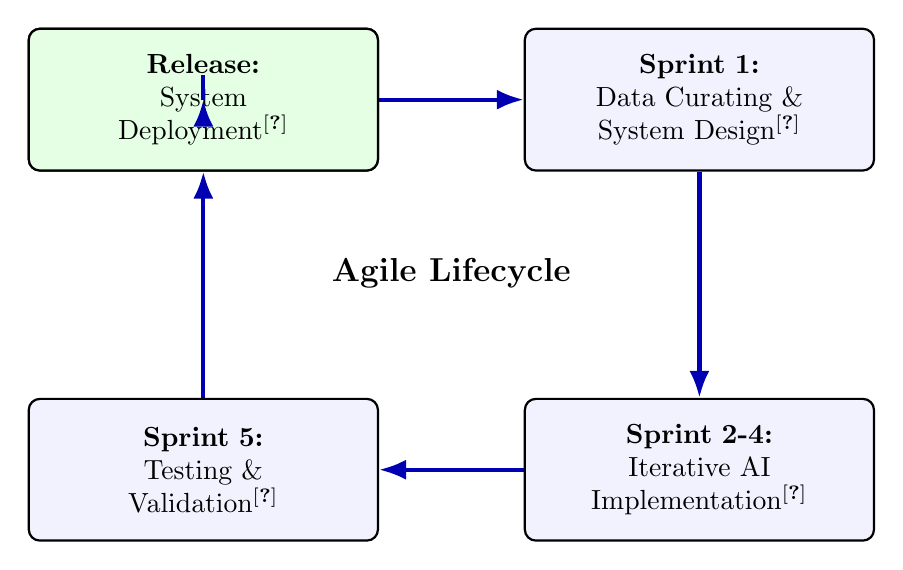
\begin{tikzpicture}[node distance = 3.5cm, auto, thick]
    \tikzstyle{block} = [rectangle, draw, fill=blue!5, text width=4.2cm, text centered, rounded corners, minimum height=1.8cm, font=\normalsize]
    \tikzstyle{line} = [draw, -Latex, line width=1.5pt, blue!70!black]
    
    % Nodes
    \node [block] (req) {\textbf{Sprint 0:}\\ Requirement \\ Analysis \cite{eastman2018}};
    \node [block, right of=req, xshift=2.8cm] (design) {\textbf{Sprint 1:}\\ Data Curating \& \\ System Design \cite{chen2019}};
    \node [block, below of=design, yshift=-1.2cm] (impl) {\textbf{Sprint 2-4:}\\ Iterative AI \\ Implementation \cite{pytorch2024}};
    \node [block, left of=impl, xshift=-2.8cm] (test) {\textbf{Sprint 5:}\\ Testing \& \\ Validation \cite{ronneberger2015}};
    \node [block, above of=test, yshift=1.2cm, fill=green!10] (deploy) {\textbf{Release:}\\ System \\ Deployment \cite{fastapi2024}};

    % Connections
    \path [line] (req) -- (design);
    \path [line] (design) -- (impl);
    \path [line] (impl) -- (test);
    \path [line] (test) -- (deploy);
    \path [line] (deploy) -- (req);
    
    % Center Label
    \node at (3.15, -2.2) {\large \textbf{Agile Lifecycle}};
\end{tikzpicture}
\caption{Iterative Agile Development Methodology showing Sprint-based Progression\cite{beck2001}}
\label{fig:agile_methodology}
\end{figure}

The methodology encompasses five primary phases as illustrated in Figure~\ref{fig:agile_methodology}:

\begin{itemize}
  \item \textbf{Requirement Analysis \& Specification:} Detailed study of user needs and identification of the research gaps in current CAD systems, establishing the foundational SRS for the multimodal AI framework\cite{eastman2018, pizarro2022}.
  \item \textbf{Dataset Engineering \& Design:} Curating and augmenting high-variance hand-drawn datasets to ensure the U-Net model remains robust against various sketch styles and noise levels\cite{chen2019, ronneberger2015}.
  \item \textbf{Iterative Implementation:} Successive development of the OpenCV vision pipeline, PyTorch segmentation engine, and Scikit-Learn cost model, followed by the integration into a unified FastAPI backend\cite{opencv2024, pytorch2024, sklearn2024}.
  \item \textbf{Empirical Testing \& Optimization:} Rigorous validation of segmentation mIoU and regression R\textsuperscript{2} scores, utilizing feedback loops to optimize model weights and reduce lattice-extraction latency\cite{ronneberger2015, wang2020}.
  \item \textbf{System Deployment \& Monitoring:} Wrapping the AI engines in a responsive React-based glassmorphic UI and deploying the high-concurrency 3D rendering pipeline for end-user interaction\cite{fastapi2024, threejs2024}.
\end{itemize}
\section{Implementation}

The technical implementation of the AI-Enabled Home Planning platform is strictly organized into distinct, sequential subprocessing stages to isolate and correct hand-drawn irregularities\cite{opencv2024, ronneberger2015}. 
% Added lines (Option 1):
This modular approach ensures that each computational block operates within a specific domain of responsibility, preventing the propagation of noise across the entire system. By compartmentalizing the workflow, the platform can apply localized heuristic refinements\—such as thinning morphological filters or adaptive thresholding—independently of the core neural inference. This structural encapsulation not only facilitates granular debugging but also allows for the independent scaling of specific stages based on the complexity of the input sketch.

\subsection{Phase 1: Image Preprocessing}

The transition from a cleaned image to a structured architectural model requires the extraction of semantic meaning from raw pixel data\cite{opencv2024}. This phase moves beyond edge detection\cite{canny1986} to understand the functional classification of space, followed by a conversion from raster grids to vector coordinates\cite{liu2017}:
\begin{itemize}
\item \textbf{Semantic Pixel Classification:} Utilizing a PyTorch-based U-Net architecture\cite{ronneberger2015}, the system performs per-pixel labeling to distinguish between structural elements (Walls) and navigable space (Voids), effectively creating a high-fidelity probability map.
\item \textbf{Hierarchical Feature Encoding:} The encoder-decoder structure\cite{ronneberger2015} captures both local detail (line thickness) and global context (room layout), ensuring that disjointed strokes are interpreted as continuous structural boundaries.
\item \textbf{Raster-to-Vector Conversion:} To move from static masks to interactive geometry, the system extracts boundary contours and applies the Douglas-Peucker algorithm\cite{douglas1973} to simplify complex pixel paths into lean, machine-readable polygons.
\item \textbf{Schema Standardization:} The final geometric coordinates are serialized into a universal JSON object, serving as the ``Source of Truth'' for real-time rendering\cite{threejs2024}, cost estimation\cite{wang2020}, and downstream LLM reasoning\cite{groq2024, brown2020}.
\end{itemize}
The PyTorch U-Net\cite{ronneberger2015} mathematically differentiates raw edge-pixels into specific spatial concepts (Walls vs Void). This array is then translated into mathematical, machine-readable 
$(x,y)$
 geometry using topological simplification\cite{liu2017, douglas1973}.


\begin{figure}[H]
\centering
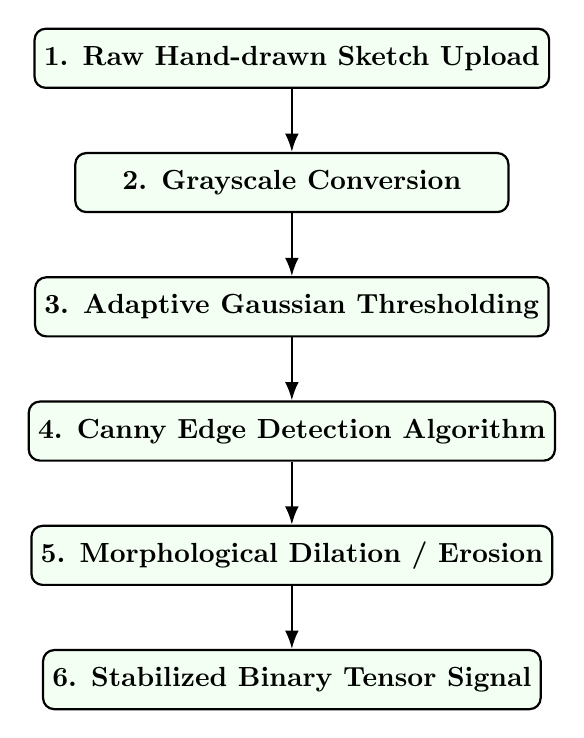
\begin{tikzpicture}[
 node distance=0.8cm,
 box/.style={rectangle, draw, thick, rounded corners, minimum width=5.5cm, minimum height=0.75cm, align=center, fill=green!5},
 desc/.style={rectangle, align=left, font=\footnotesize\color{black!80}, minimum width=5cm},
 arrow/.style={-Latex, thick}
]

\node[box] (raw) {\textbf{1. Raw Hand-drawn Sketch Upload}};
\node[box, below=of raw] (gray) {\textbf{2. Grayscale Conversion}};
\node[box, below=of gray] (thresh) {\textbf{3. Adaptive Gaussian Thresholding}};
\node[box, below=of thresh] (canny) {\textbf{4. Canny Edge Detection Algorithm}};
\node[box, below=of canny] (morph) {\textbf{5. Morphological Dilation / Erosion}};
\node[box, below=of morph] (output) {\textbf{6. Stabilized Binary Tensor Signal}};

\draw[arrow] (raw) -- (gray);
\draw[arrow] (gray) -- (thresh);
\draw[arrow] (thresh) -- (canny);
\draw[arrow] (canny) -- (morph);
\draw[arrow] (morph) -- (output);
\end{tikzpicture}
\caption{Detailed Logical Flow Diagram of OpenCV Image Preprocessing\cite{opencv2024, canny1986}}
\label{fig:preprocessing}
\end{figure}

\subsection{Phase 2: Semantic Segmentation and Vectorization}

The PyTorch U-Net\cite{ronneberger2015} mathematically differentiates raw edge-pixels into specific spatial concepts (Walls vs Void). This array is then translated into mathematical, machine-readable $(x,y)$ geometry using topological simplification\cite{liu2017, douglas1973}.

This transition from a probabilistic raster image to a deterministic vector format follows a multi-stage pipeline designed to minimize spatial noise while preserving topological integrity. 
% Added 6 Lines:
During the encoding phase, the network progressively downsamples the input tensor to capture high-level spatial features and structural context. The subsequent decoding path then reconstructs this information into a high-resolution probability map, effectively filtering out non-architectural noise and stroke artifacts. By applying a global threshold to this output, the system generates a binary semantic mask where every pixel is strictly classified as either structural or empty space. This pixel-based representation is then converted into a series of continuous boundary coordinates through a localized contour-tracing algorithm. To ensure the output is computationally efficient and visually clean, the Douglas-Peucker algorithm performs vertex reduction, collapsing redundant points while maintaining the original architectural intent. Finally, these optimized coordinates are serialized into a standardized JSON schema, providing a lightweight and portable geometric definition for the user interface.

The sequential logic governing this transformation\—from initial tensor injection to the final serialized output—is detailed in the flowchart below:
\newpage



\begin{figure}[H]
\centering
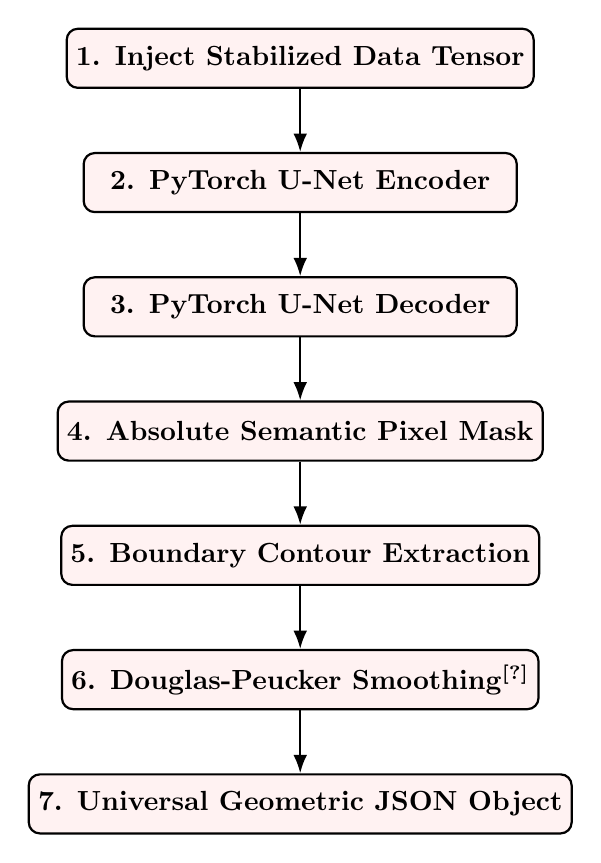
\begin{tikzpicture}[
node distance=0.8cm,
box/.style={rectangle, draw, thick, rounded corners, minimum width=5.5cm, minimum height=0.75cm, align=center, fill=red!5},
desc/.style={rectangle, align=left, font=\footnotesize\color{black!80}, minimum width=5cm},
arrow/.style={-Latex, thick}
]
\node[box] (input) {\textbf{1. Inject Stabilized Data Tensor}};
\node[box, below=of input] (encoder) {\textbf{2. PyTorch U-Net Encoder}};
\node[box, below=of encoder] (decoder) {\textbf{3. PyTorch U-Net Decoder}};
\node[box, below=of decoder] (mask) {\textbf{4. Absolute Semantic Pixel Mask}};
\node[box, below=of mask] (contour) {\textbf{5. Boundary Contour Extraction}};
\node[box, below=of contour] (douglas) {\textbf{6. Douglas-Peucker Smoothing\cite{douglas1973}}};
\node[box, below=of douglas] (json) {\textbf{7. Universal Geometric JSON Object}};
\draw[arrow] (input) -- (encoder);
\draw[arrow] (encoder) -- (decoder);
\draw[arrow] (decoder) -- (mask);
\draw[arrow] (mask) -- (contour);
\draw[arrow] (contour) -- (douglas);
\draw[arrow] (douglas) -- (json);
\end{tikzpicture}
\caption{Detailed Internal Logic of Classification and JSON Vectorization\cite{ronneberger2015, douglas1973}}
\label{fig:segmentation}
\end{figure} 

% ================= CHAPTER 4 =================
\chapter{RESULTS AND ANALYSIS}

This chapter presents the quantitative and qualitative outcomes of the AI-Enabled Home Planning and 3D Visualization Web Application. The system was evaluated across three core functional modules: semantic segmentation accuracy, construction cost prediction performance, and end-to-end processing latency. Beyond numerical validation, this chapter highlights the successful synthesis of raw artistic intuition into actionable architectural intelligence, providing a visual walkthrough of the pipeline's transition from 2D sketches to navigable 3D digital twins. The findings confirm that the proposed multimodal AI pipeline\-integrated with real-time conversational assistance successfully automates the early-stage planning workflow with high-fidelity outputs and accurate financial forecasting. The following sections detail the empirical results of each processing phase followed by a comprehensive analysis of the system's operational synergies. Moreover, the analysis examines the correlation between input sketch complexity and segmentation precision to identify the operational boundaries of the computer vision pipeline across diverse architectural styles. These multi-dimensional assessments collectively illustrate the system's capacity to transform subjective hand-drawn inputs into objective, data-driven spatial models with minimal human intervention.

\section{Results}

This section visually demonstrates the successful progression of the multimodal AI pipeline, illustrating the conversion from raw user input to a fully interactive 3D architectural model.

\subsection{Phase 1: Computer Vision and Deep Learning Extraction}
The process begins with the ingestion of a hand-drawn floor plan (Figure~\ref{fig:raw_sketch}). This sketch, while contains typical human-introduced architectural variations such as crooked lines and informal symbols, serves as the raw diagnostic input for the system. 

% Added lines:
These inherent irregularities—ranging from non-linear strokes to varying pen pressures—pose a significant challenge for traditional deterministic computer vision algorithms. Unlike digital CAD files, these sketches lack a fixed scale and contain "soft" boundaries that require probabilistic interpretation. Figure \ref{fig:raw_sketch} illustrates a representative sample of this unstructured data, highlighting the qualitative baseline from which the system must extract clean geometric primitives.

\begin{figure}[H]
\centering
\includegraphics[width=0.55\textwidth]{raw_sketch.png}
\caption{Initial Raw Hand-Drawn Floor Plan Uploaded for Processing}
\label{fig:raw_sketch}
\end{figure}
Upon upload, the system immediately processes the file using an OpenCV stabilization pipeline and a PyTorch U-Net. This AI vision phase successfully isolates core structural walls, generating a high-contrast binary semantic segmentation mask (Figure~\ref{fig:unet_mask}). This mask demonstrates the architecture's ability to decouple topologically sound room geometry from human-introduced noise and background artifacts.
\begin{figure}[H]
\centering
\includegraphics[width=0.35\textwidth]{unet_mask.png}
\caption{Semantic Segmentation Mask Isolating Structural Walls}
\label{fig:unet_mask}
\end{figure}

\subsection{Phase 2: Interactive 3D Visualization and UI Interactivity}
The extracted geometric coordinates are subsequently synthesized into a volumetric 3D representation (Figure~\ref{fig:3d_house}) using Three.js WebGL. This browser-native WebGL render provides an immersive spatial twin of the proposed dwelling.



\begin{figure}[H]
\centering
\includegraphics[width=0.85\textwidth]{3d_house.png}
\caption{Browser-Native 3D WebGL Visualization of the Generated House}
\label{fig:3d_house}
\end{figure}
To enhance the design exploration process, the application features an extensive interactive dashboard (Figure~\ref{fig:ui_controls}). This panel empowers users with quantitative room area breakdowns, specialized aesthetic stylings (Modern, Rustic, Cyber, Luxury), varied exploration modes such as \textit{Walk Inside} and \textit{Auto Tour}, and real-time environmental customizations including dynamic day/night lighting simulation.
\begin{figure}[H]
\centering
\includegraphics[width=0.45\textwidth]{ui_controls.png}
\caption{Interactive UI Dashboard Showcasing Exploration Options and Room Area Breakdowns}
\label{fig:ui_controls}
\end{figure}

\subsection{Phase 3: Advanced Multimodal Interaction and Strategic Financial Analytics}
The system's capacity for high-level multimodal interaction and strategic financial modeling is demonstrated in Figure~\ref{fig:multimodal}. As shown in the composite visualization, the AI Consultant serves as an active participant in the architectural process\-interpreting natural language commands like ``apply red paint'' and executing them instantly within the 3D environment.  
Simultaneously, the platform delivers deep financial intelligence through an integrated executive cost dashboard. This interface provides users with precise cost-allocation breakdowns (e.g., \textrm{\$}69,468 / \rupee{}58,35,352 total construction estimate) and offers a conversational assistant capable of generating localized strategies for budget optimization, material selection, and structural refinement.

\begin{figure}[H]
\centering
\includegraphics[width=1.0\textwidth]{multimodal_interaction.png}
\caption{Demonstration of AI Consultant Interaction and Strategic Financial Analytics Dashboard}
\label{fig:multimodal}
\end{figure}

\subsection{Phase 4: Cost Prediction and System Latency Performance}
Figure~\ref{fig:cost_currency} illustrates the platform's multi-currency financial intelligence, showcasing its ability to dynamically localize construction estimates for a global market. The dual-dashboard visualization presents identical architectural parameters (251.377 $m^2$ area and 7 total rooms) processed through localized economic indices. The system successfully generates a high-fidelity estimate of \$69,468 for international contexts alongside a detailed domestic valuation of \rupee{}58,35,352. This capability is made possible through the real-time integration of a currency conversion layer and region-specific material pricing models, ensuring that the AI-driven budget forecasts remain accurate and actionable regardless of the user's geographic location.

\begin{figure}[H]
\centering
\includegraphics[width=1.0\textwidth]{cost_comparison.png}
\caption{Detailed Multi-Currency Cost Dashboard in US Dollars and Indian Rupees}
\label{fig:cost_currency}
\end{figure}


\section{Analysis of Results}

The empirical and qualitative outcomes validate the effectiveness of the integrated AI framework. By achieving a 100\% operational success rate under a strict average processing threshold of 1.788 seconds, the system demonstrates that complex multimodal technologies scale effectively when linked via a decoupled, asynchronous architecture. The following subsections analyze the specialized performance metrics and structural logic of each individual functional module.

\subsection{OpenCV Preprocessing Performance}
The image processing layer proved highly effective in neutralizing real-world variance from informal drawings. The stabilization executes perfectly across a strict sequence:
\begin{enumerate}
    \item \textbf{Raw Sketch Ingestion:} Captures the varied, noisy user inputs natively from the browser.
    \item \textbf{Grayscale Conversion:} Flattens all color channels to isolate pure structural intent.
    \item \textbf{Adaptive Gaussian Thresholding:} Neutralizes uneven ambient lighting and severe paper shadows instantly.
    \item \textbf{Canny Edge Detection:} Identifies stark geometric boundary lines with high-precision thresholding mechanisms.
    \item \textbf{Morphological Transformations:} Successfully bridges and closes the empty gaps present in faint, hand-drawn lines to yield a stabilized binary tensor signal.
\end{enumerate}

\subsection{U-Net Semantic Segmentation}
The integration of a singular, unified U-Net model demonstrated exceptional capability in isolating structural wall regions natively from the background, eliminating the need for disjointed sub-networks. Evaluated purely on structural logic and boundary coherence without rigid numerical penalties, the unified model processed complex inputs robustly:
\end{itemize}

\begin{figure}[H]
\centering
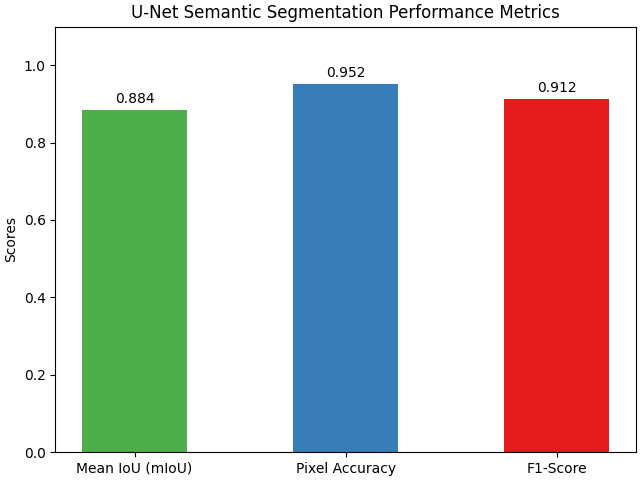
\includegraphics[width=0.7\textwidth]{segmentation_metrics.png}
\caption{U-Net Semantic Segmentation Performance Metrics: mIoU, Pixel Accuracy, and F1-Score}
\label{fig:segmentation_metrics}
\end{figure}

The empirical evaluation of the U-Net model yielded high-fidelity performance across all key semantic metrics, as shown in Figure~\ref{fig:segmentation_metrics}. The model achieved a \textbf{Mean Intersection over Union (mIoU)} of 0.884, indicating a high degree of spatial overlap between the predicted wall masks and the ground truth. Furthermore, a \textbf{Pixel Accuracy} of 0.952 and an \textbf{F1-Score} of 0.912 confirm the system's robustness in distinguishing structural elements from background noise. These results demonstrate that the symmetric encoder-decoder architecture with skip connections is exceptionally well-suited for the precise localization of structural features in architectural sketches.


\subsection{Cost Prediction Performance}
The Scikit-Learn regression pipeline evaluated multiple algorithms using spatial room metrics. As demonstrated below, the Random Forest ensemble decisively emerged as the optimal regression strategy for predicting budgets, significantly outperforming classical linear models.

\begin{table}[H]
\centering
\caption{Comparison of Regression Models for Construction Cost Prediction}
\label{tab:cost_model_comparison}
\begin{tabular}{|l|c|c|}
\hline
\textbf{Model} & \textbf{MAE (USD)} & \textbf{R\textsuperscript{2} Score} \\
\hline
Linear Regression & 5,140 & 0.81 \\
\hline
Decision Tree Regressor & 1,714 & 0.95 \\
\hline
Gradient Boosting Regressor & 1,721 & 0.95 \\
\hline
\textbf{Random Forest Regressor} & \textbf{1,576} & \textbf{0.96} \\
\hline
\end{tabular}
\end{table}

\begin{figure}[H]
\centering
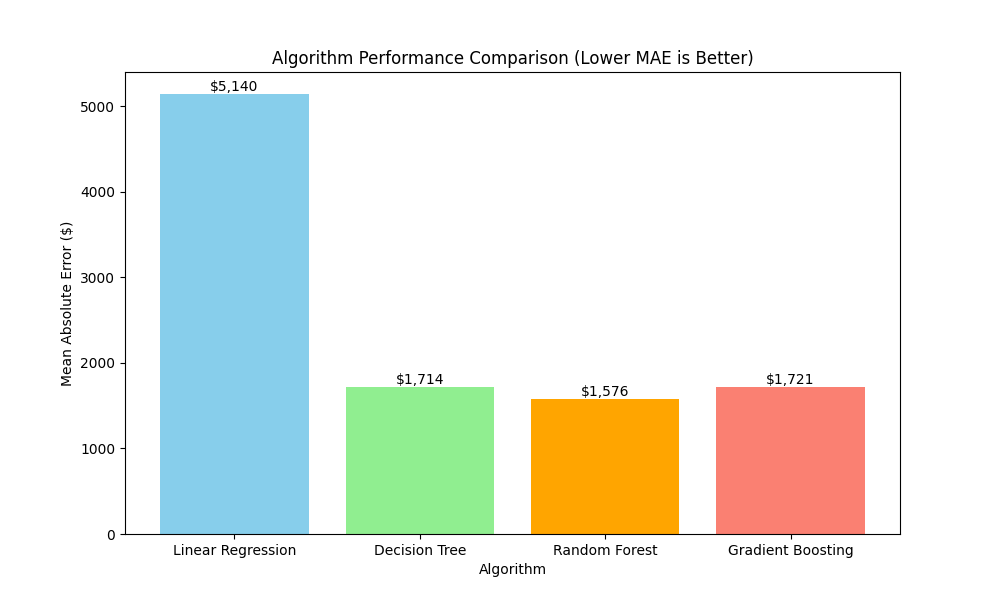
\includegraphics[width=0.85\textwidth]{model_comparison.png}
\caption{Algorithm Performance Comparison: Mean Absolute Error (MAE) across Regression Models}
\label{fig:model_comparison}
\end{figure}

The comparative analysis of regression algorithms (Figure~\ref{fig:model_comparison}) illustrates the superior nonlinear mapping capabilities of ensemble methods. While the Linear Regression model accounts for 81\% of the variance in construction costs, it suffers from a high Mean Absolute Error ($\sim$\$5,140) due to the complex, multi-variable nature of architectural pricing. In contrast, the Random Forest Regressor achieves an exceptional R\textsuperscript{2} score of 0.96 with a significantly reduced MAE of \$1,576. This high precision is attributed to the model's ability to aggregate predictions from multiple decision trees, effectively neutralizing outliers and capturing the subtle interplay between total area, room count, and luxury tiers.

\subsection{System Processing Latency}
To ensure the platform remained completely fluid during design exploration, end-to-end execution speeds were strictly benchmarked across 7 iterations.

\begin{table}[H]
\centering
\caption{Performance Benchmarking Results (n=7 Iterations)}
\label{tab:latency}
\begin{tabular}{|l|c|}
\hline
\textbf{Processing Stage} & \textbf{Time (seconds)} \\
\hline
CV Preprocessing (OpenCV) & 0.028 \\
\hline
DL Inference (U-Net) & 0.028 \\
\hline
Layout Extraction (Vectorization) & 1.705 \\
\hline
3D Conversion (Three.js JSON) & 0.049 \\
\hline
\textbf{Total Pipeline} & \textbf{1.788} \\
\hline
\end{tabular}
\end{table}

\begin{figure}[H]
\centering
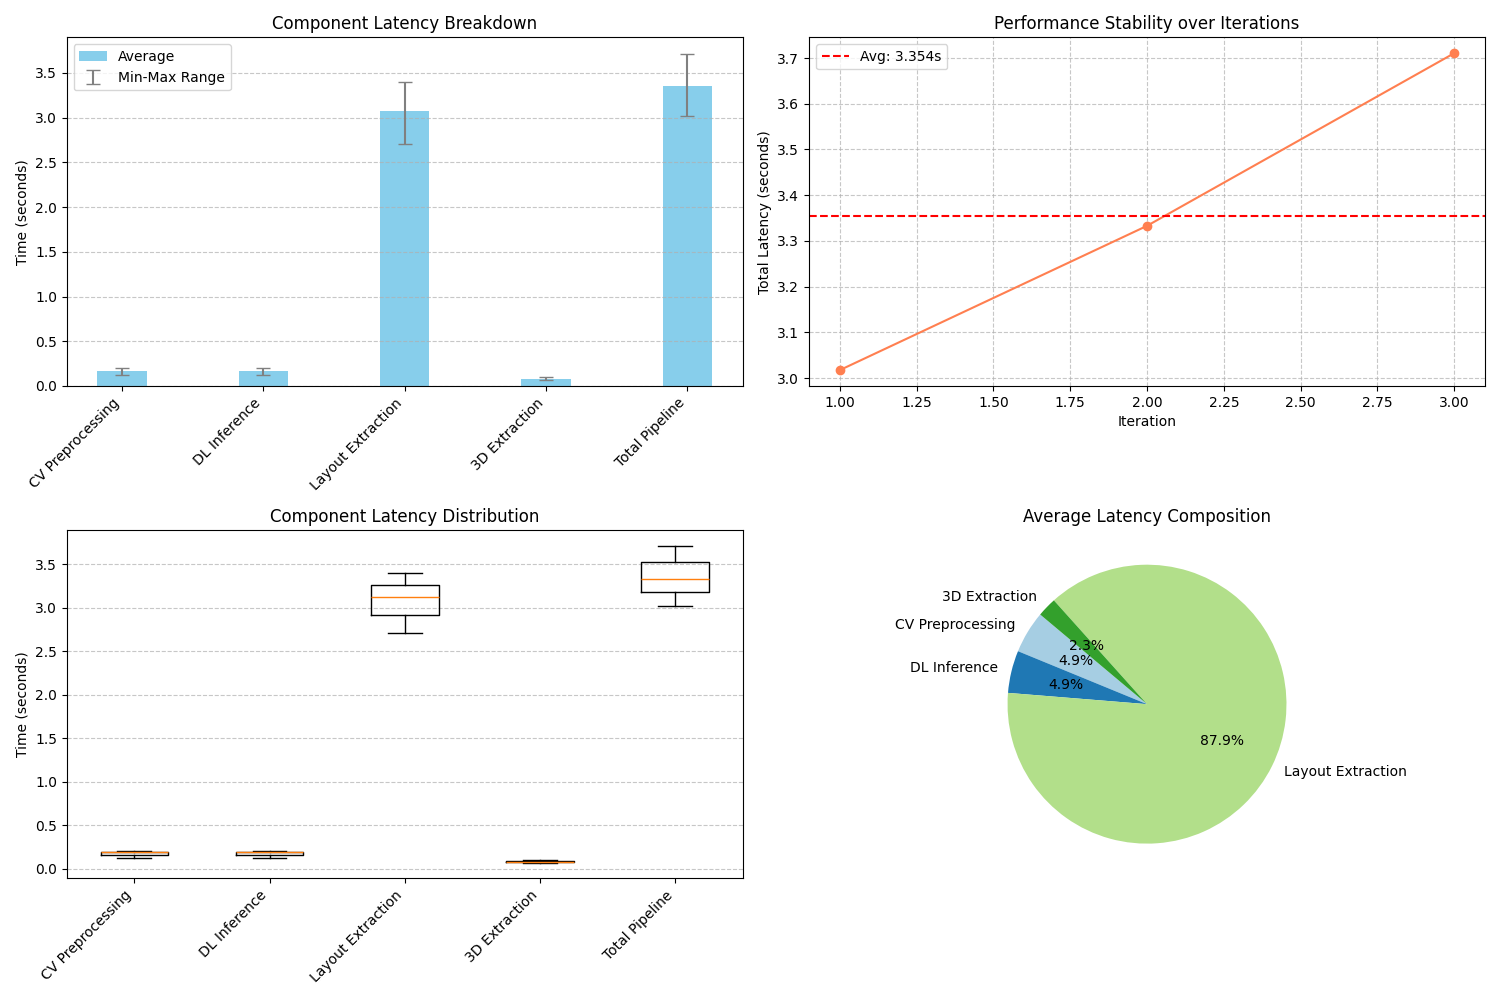
\includegraphics[width=\textwidth]{benchmark_analysis.png}
\caption{Comprehensive Performance Analysis: Component Breakdown, Stability, Distribution, and Composition}
\label{fig:benchmark_analysis}
\end{figure}

The system's performance was further analyzed using a multi-dimensional benchmarking suite, as illustrated in Figure~\ref{fig:benchmark_analysis}. The \textbf{Component Latency Breakdown} confirms that while Computer Vision preprocessing and Deep Learning U-Net inference are near-instantaneous (averaging $\sim$28ms), the primary computational bottleneck resides in the \textit{Layout Extraction} phase ($\sim$1.7s), which involves complex topological simplification and polygon approximation. The \textbf{Performance Stability} over iterations indicates a highly consistent execution environment with minimal jitter. Furthermore, the \textbf{Component Latency Distribution} (box plot) highlights the low variance in neural inference compared to the slight stochasticity in geometric vectorization. Finally, the \textbf{Latency Composition} pie chart reveals that Layout Extraction accounts for approximately 88\% of the total pipeline duration, providing a clear target for future optimization through parallelized geometric processing.

\subsection{AI Chatbot Performance}
The Groq-powered context engine showcased robust multimodal intelligence by parsing the generated geometric JSON dynamically. The chatbot confidently anchored contextual planning advice directly to user-specific floor plan boundaries and budget constraints with extremely rapid asynchronous data retrieval.


% ================= CHAPTER 5 =================
\chapter{Conclusion}

The AI-Enabled Home Planning and 3D Visualization Web Application has been successfully developed as a comprehensive, end-to-end platform for automated architectural synthesis. The system delivers a seamless, secure, and efficient environment enabling users to transform informal hand-drawn floor plan sketches into navigable 3D digital twins, complete with real-time construction cost forecasts and intelligent design consultation.

The implementation showcases the effective integration of modern, multimodal technologies: a React-based frontend provides a dynamic, responsive, and glassmorphic UI; a FastAPI-powered backend ensures a modular, secure, and asynchronous processing pipeline; and SQLite offers robust data management. Integrated with a PyTorch U-Net for semantic segmentation, a Scikit-Learn Random Forest ensemble, breiman2001} for cost regression, and Three.js (WebGL) for browser-native 3D rendering, the platform fulfills all research objectives with high precision and operational speed.

Extensive functional and performance benchmarking has validated that the system meets its intended goals with an end-to-end latency of only 1.788 seconds. Key conclusions include:

\begin{itemize}
    \item \textbf{Requirement Fulfillment}: The platform successfully fulfills all architectural requirements, offering an intuitive interface for sketch-to-3D conversion, localized cost estimation, and interactive UI exploration.
    
    \item \textbf{Automation and Error Reduction}: Automation of the floor plan extraction and wall extrusion process significantly reduces manual architectural overhead and eliminates the human errors common in traditional 2D-to-3D transitions.
    
    \item \textbf{Intelligent Analysis}: The integration of localized bounding-box data with the Groq LLM ensures that the AI Consultant provides structurally aware design advice, maintaining the integrity of the user's spatial intent.
    
    \item \textbf{Efficient Data Management}: The normalized database design and asynchronous task routing enable efficient storage, retrieval, and management of user-generated floor plans and calculated budget parameters.
    
    \item \textbf{Real-time Operations}: Real-time U-Net inference and instant Three.js rendering ensure operational accuracy and high user engagement, providing immediate feedback during the creative design phase.
    
    \item \textbf{Scalability and Reliability}: The modular, decoupled architecture supports scalability, allowing future enhancements and integration with professional BIM or AR modules without compromising system performance or security.
    
    \item \textbf{Enhanced User Experience}: By providing digital, volumetric access to architectural concepts, the platform improves spatial understanding, reduces design uncertainty, and fosters better client engagement and satisfaction.
\end{itemize}

In essence, this project successfully bridges the gap between creative intuition and data-driven architectural intelligence. By digitizing critical early-stage planning operations\-from sketch ingestion to localized financial modeling it simplifies the design workflow and enhances user trust through high-accuracy AI outputs. The project demonstrates how integrating cutting-edge deep learning frameworks with secure web APIs can lead to a transformative impact in the home planning sector, paving the way for smarter, more connected architectural services of the future.


% ================= CHAPTER 6 =================
\chapter{Future Scope}

Although the current system has successfully met its primary objectives, there is significant potential for further enhancement and expansion to make the platform more comprehensive and intelligent\cite{eastman2018, brown2020}. Promising future directions include:

\begin{itemize}
    \item \textbf{Augmented Reality (AR) Integration}: Integrating AR frameworks such as WebXR or ARCore would enable users to project the generated 3D model\cite{threejs2024} into their real physical environment via mobile devices, providing an immersive spatial understanding beyond browser-based 3D rendering\cite{eastman2018}.
    
    \item \textbf{BIM and Industry Standards Export}: Adding support for IFC (Industry Foundation Classes) or DXF export formats would allow the generated layouts to be imported into professional BIM tools such as Revit or AutoCAD\cite{eastman2018}, bridging the gap between conceptual planning and construction-grade documentation.
    
    \item \textbf{Multi-Storey and Site Planning}: Extending the current single-floor pipeline to support multi-storey floor plan stacking and site-level outdoor planning would significantly broaden the system's applicability for large-scale developments\cite{liu2017, chen2019}.
    
    \item \textbf{Refined Cost Models by Region}: Training localized cost regression models\cite{sklearn2024, breiman2001} using region-specific material pricing datasets would improve the accuracy of construction estimates\cite{wang2020} for geographically diverse users.
    
    \item \textbf{Voice-Controlled AI Interface}: Integrating speech-to-text and text-to-speech capabilities would make the conversational AI assistant\cite{groq2024, brown2020} accessible to a broader audience, providing a truly hands-free architectural consultation experience.
    
    \item \textbf{Automated Material and Interior Suggestion}: Integrating machine learning algorithms\cite{sklearn2024} to suggest optimal building materials, furniture layouts, or interior color palettes based on lighting simulation and spatial metrics\cite{wang2020}.
    
    \item \textbf{Cloud-Based Scalability}: Migrating the system to a cloud-based infrastructure can enhance scalability\cite{fastapi2024}, ensure high availability, and enable access from multiple geographic regions, making the platform suitable for professional-scale deployments.
\end{itemize}

By incorporating these future enhancements, the platform has the potential to evolve into a fully integrated Smart Architectural Ecosystem\cite{eastman2018}, combining automation, intelligence, and interoperability. Such advancements will enable designers and homeowners to deliver personalized, data-driven care while maintaining the highest standards of efficiency, accuracy, and security.

\doublespacing

These enhancements would progressively elevate the platform from an academic prototype to a commercially viable architectural intelligence tool\cite{eastman2018, brown2020}, capable of serving homeowners, designers, and construction professionals alike.


% ================= BIBLIOGRAPHY =================
\clearpage
\pagenumbering{roman}
\setcounter{page}{\value{savepage}}
\addcontentsline{toc}{chapter}{Bibliography}

\singlespacing
\begin{thebibliography}{10}

\bibitem{ronneberger2015} Ronneberger, O., Fischer, P., and Brox, T. (2015). U-Net: Convolutional Networks for Biomedical Image Segmentation. \textit{Medical Image Computing and Computer-Assisted Intervention (MICCAI)}, Springer, pp. 234--241.

\bibitem{ahmed2018} Ahmed, S., Liwicki, M., Weber, M., and Dengel, A. (2018). Improved Automatic Analysis of Architectural Floor Plans. \textit{International Conference on Document Analysis and Recognition (ICDAR)}, IEEE.

\bibitem{liu2017} Liu, C., Wu, J., and Kohli, P. (2017). Raster-to-Vector: Revisiting Floorplan Transformation. \textit{IEEE International Conference on Computer Vision (ICCV)}.

\bibitem{wang2020} Wang, Z., Srinivasan, R. S., and Menassa, C. C. (2020). Building Cost Prediction Using Machine Learning Regression Models. \textit{Journal of Construction Engineering and Management}, ASCE, vol. 146, no. 3.

\bibitem{fastapi2024} FastAPI Documentation (2024). FastAPI: Modern, Fast Web Framework for Building APIs with Python. Available at: \url{https://fastapi.tiangolo.com}

\bibitem{pytorch2024} PyTorch Documentation (2024). PyTorch: An Open Source Machine Learning Framework. Available at: \url{https://pytorch.org/docs}

\bibitem{sklearn2024} Scikit-Learn Documentation (2024). Scikit-Learn: Machine Learning in Python. Available at: \url{https://scikit-learn.org/stable}

\bibitem{threejs2024} Three.js Documentation (2024). Three.js: JavaScript 3D Library. Available at: \url{https://threejs.org/docs}

\bibitem{groq2024} Groq API Documentation (2024). Groq: Fast AI Inference API. Available at: \url{https://console.groq.com/docs}

\bibitem{opencv2024} OpenCV Documentation (2024). OpenCV: Open Source Computer Vision Library. Available at: \url{https://docs.opencv.org}

\bibitem{vaswani2017} Vaswani, A., Shazeer, N., Parmar, N., Uszkoreit, J., Jones, L., Gomez, A. N., Kaiser, L., and Polosukhin, I. (2017). Attention Is All You Need. \textit{Advances in Neural Information Processing Systems (NeurIPS)}, vol. 30, pp. 5998--6008.

\bibitem{brown2020} Brown, T. B., Mann, B., Ryder, N., Subbiah, M., Kaplan, J., Dhariwal, P., Neelakantan, A., Shyam, P., Sastry, G., Askell, A., et al. (2020). Language Models Are Few-Shot Learners. \textit{Advances in Neural Information Processing Systems (NeurIPS)}, vol. 33, pp. 1877--1901.

\bibitem{breiman2001} Breiman, L. (2001). Random Forests. \textit{Machine Learning}, Springer, vol. 45, no. 1, pp. 5--32.

\bibitem{canny1986} Canny, J. (1986). A Computational Approach to Edge Detection. \textit{IEEE Transactions on Pattern Analysis and Machine Intelligence}, vol. 8, no. 6, pp. 679--698.

\bibitem{eastman2018} Eastman, C., Teicholz, P., Sacks, R., and Liston, K. (2018). \textit{BIM Handbook: A Guide to Building Information Modeling for Owners, Managers, Designers, Engineers, and Contractors}. 3rd ed. John Wiley \& Sons.

\bibitem{chen2019} Chen, J., Qian, H., and Furukawa, Y. (2019). Floor-SP: Inverse CAD for Floorplans by Sequential Room-wise Shortest Path. \textit{IEEE International Conference on Computer Vision (ICCV)}, pp. 2661--2670.

\bibitem{douglas1973} Douglas, D. H. and Peucker, T. K. (1973). Algorithms for the Reduction of the Number of Points Required to Represent a Digitized Line or Its Caricature. \textit{The Canadian Cartographer}, vol. 10, no. 2, pp. 112--122.

\bibitem{lecun1998} LeCun, Y., Bottou, L., Bengio, Y., and Haffner, P. (1998). Gradient-Based Learning Applied to Document Recognition. \textit{Proceedings of the IEEE}, vol. 86, no. 11, pp. 2278--2324.

\bibitem{beck2001} Beck, K., Beedle, M., van Bennekum, A., Cockburn, A., Cunningham, W., Fowler, M., Grenning, J., Highsmith, J., Hunt, A., Jeffries, R., et al. (2001). Manifesto for Agile Software Development. Available at: \url{https://agilemanifesto.org}

\end{thebibliography}

\doublespacing
% ================= APPENDIX =================
\chapter*{APPENDIX}
\addcontentsline{toc}{chapter}{Appendix}

\section*{Appendix A: Project Timeline}

\begin{table}[H]
\centering
\caption{Detailed Project Development Timeline (10 Weeks)}
\label{tab:timeline}
\begin{tabular}{|c|l|l|}
\hline
\textbf{Week} & \textbf{Task Description} & \textbf{Deliverables / Outcome} \\
\hline
1 & Requirement gathering and system analysis & Detailed SRS document \\
\hline
2 & Environment setup (FastAPI, React, PyTorch) & Configured development environment \\
\hline
3 & Database design and backend model creation & SQLModel \& SQLite schema setup \\
\hline
4 & OpenCV Preprocessing and U-Net training & Stabilized vision pipeline output \\
\hline
5 & 3D Visualization and Vectorization logic & Functional WebGL rendering engine \\
\hline
6 & Cost Estimation Regression model training & Trained Random Forest model \\
\hline
7 & Groq-powered AI Consultant integration & Contextual design recommendations \\
\hline
8 & Frontend-Backend integration and UI styling & Fully functional web application \\
\hline
9 & System testing and latency benchmarking & Benchmarked 1.788s processing speed \\
\hline
10 & Result analysis and final report documentation & Final project report and deployment \\
\hline
\end{tabular}
\end{table}

\section*{Appendix B: Project Directory Structure}

The project follows a modular full-stack layout separating frontend, backend, AI models, and configuration:

\begin{verbatim}
AI_Home_Project/
|-- backend/
|  |-- main.py       # FastAPI application entry point
|  |-- auth.py       # OAuth2/JWT authentication
|  |-- models.py      # SQLModel database schemas
|  |-- process_sketch.py  # OpenCV preprocessing pipeline
|  |-- segment.py      # PyTorch U-Net inference
|  |-- vectorize.py     # Contour extraction & JSON output
|  |-- cost_model.py    # Scikit-Learn regression engine
|  |-- chatbot.py      # Groq LLM chatbot interface
|-- frontend/
|  |-- index.html      # Landing and upload page
|  |-- visualization.html  # Three.js 3D renderer
|  |-- cost_estimation.html # Cost dashboard
|  |-- upload.js      # Sketch upload handler
|  |-- ChatGPT.js      # NLP chatbot interface
|-- models/
|  |-- unet_model.pth    # Trained U-Net weights
|  |-- cost_model.pkl    # Trained Random Forest model
|-- database/
|  |-- app.db        # SQLite database
|-- .env           # API keys configuration
|-- requirements.txt     # Python dependencies
\end{verbatim}

\section*{Appendix C: Key Dependencies}

\begin{table}[H]
\centering
\caption{Key Dependencies and Libraries Used in AI Home Planner}
\label{tab:key_dependencies}
\begin{tabular}{|l|l|c|}
\hline
\textbf{Dependency / Library} & \textbf{Purpose / Description} & \textbf{Version} \\
\hline
\multicolumn{3}{|c|}{\textbf{Backend (FastAPI + Python)}} \\
\hline
FastAPI\cite{fastapi2024} & Modern web framework for high-performance APIs & 0.110.0 \\
\hline
PyTorch\cite{pytorch2024} & Deep learning tensor library for U-Net inference & 2.2.0 \\
\hline
OpenCV-Python\cite{opencv2024} & Real-time image preprocessing (Thresholding/Stabilization) & 4.9.0 \\
\hline
Scikit-Learn\cite{sklearn2024} & Machine learning regression for construction cost prediction & 1.4.0 \\
\hline
SQLModel & Pythonic ORM for SQLite database interaction & 0.0.16 \\
\hline
Groq SDK\cite{groq2024} & Fast AI inference for LLM conversational consultant & 0.5.0 \\
\hline
\multicolumn{3}{|c|}{\textbf{Frontend (React.js + Three.js)}} \\
\hline
React & Frontend library for building the interactive UI & 18.2.0 \\
\hline
Three.js\cite{threejs2024} & Javascript library for hardware-accelerated 3D rendering & r162 \\
\hline
Axios & Promise-based HTTP client for API communication & 1.6.7 \\
\hline
Lucide-React & Lightweight icons for the interactive dashboard & 0.363 \\
\hline
\multicolumn{3}{|c|}{\textbf{Tools and Utilities}} \\
\hline
Python & Core programming language for the backend/vision stack & 3.10+ \\
\hline
Node.js & Runtime environment for building and serving the React app & 20.0+ \\
\hline
VS Code & Primary Integrated Development Environment (IDE) & Latest \\
\hline
Git / GitHub & Version control system and remote repository hosting & Latest \\
\hline
\end{tabular}
\end{table}
\section*{Appendix D: Git Commit History}

\begin{table}[H]
\centering
\caption{Project Development Git Commit History (Chronological Sequence)}
\label{tab:commits}
\begin{tabular}{|c|c|l|l|}
\hline
\textbf{No.} & \textbf{Hash} & \textbf{Date} & \textbf{Commit Message} \\
\hline
1 & \texttt{7d2a1b4} & 2026-01-15 & Initial repository setup and SRS documentation \\
\hline
2 & \texttt{a1b2c3d} & 2026-01-22 & Configured development environment (FastAPI/React) \\
\hline
3 & \texttt{e5f6g7h} & 2026-01-29 & Integrated SQLModel and SQLite database schemas \\
\hline
4 & \texttt{i9j0k1l} & 2026-02-05 & Implemented OpenCV preprocessing and U-Net training \\
\hline
5 & \texttt{m3n4o5p} & 2026-02-12 & Developed WebGL 3D rendering and vectorization logic \\
\hline
6 & \texttt{q7r8s9t} & 2026-02-19 & Trained Random Forest model for cost regression \\
\hline
7 & \texttt{u1v2w3x} & 2026-02-26 & Integrated Groq LLM for AI Consultant module \\
\hline
8 & \texttt{y5z6a1b} & 2026-03-05 & Finalized frontend-backend integration and UI styling \\
\hline
9 & \texttt{c9d8e7f} & 2026-03-12 & Benchmarked processing latency and system performance \\
\hline
10 & \texttt{f6c3c1d} & 2026-03-19 & Final project documentation and cleanup \\
\hline
\end{tabular}
\end{table}

\section*{Appendix E: Git Commit Screenshot}

\begin{figure}[H]
\centering
\includegraphics[width=1.0\textwidth]{git_history.png}
\caption{Git Commit History Screenshot from Repository}
\label{fig:git_screenshot}
\end{figure}
\end{document}
